\documentclass[
a4paper,   
headsepline, 
fleqn,     
11pt
]{scrartcl}

%%% ngerman: language set to new-german
\usepackage{ngerman}
\usepackage[utf8]{inputenc}
\usepackage[T1]{fontenc}
\usepackage{ae,aecompl}

%%% Graphic stuff
\usepackage{graphicx}
\usepackage{geometry}
\geometry{verbose,a4paper,tmargin=25mm,bmargin=25mm,lmargin=15mm,rmargin=20mm}
\usepackage{amsmath,amssymb,amstext}
\usepackage{units}
\usepackage{scrpage2}

%%% comments, ...
\usepackage{verbatim}

\setlength{\parindent}{0em} 

\renewcommand*\thesection{\Alph{section}}

\newcommand{\mygraphics}[3]{
  \begin{center}
    \includegraphics[width=#1, keepaspectratio=true]{#2} \\
    \textbf{#3}
  \end{center}
}

%%%      footer - middle: page number
\pagestyle{scrheadings}

%%% heading - left
 \ihead[]{Marco Sohm, Kevin Wallis}

%%% heading - right
 \ohead[]{Aufgabe 3}

\begin{document}

 \pagenumbering{roman} %% small roman page numbers
 \pagenumbering{arabic} 

\section{Modellieren des Systems in AnyLogic}
Das System wurde laut Angabe in AnyLogic modelliert. Wenn nicht anders angegeben, dann wurden die Default-Werte laut Angabe verwendet (Terminals $=10$, Denkzeit im Mittel $=25s$, Maximale Rechenzeit $=0.1s$, Overhead swapping $=0.015s$, Mittlere CPU Zeit $=0.8s$).
Die mittlere Denkzeit und die mittlere Zeit an CPU Bedarf kann als Parameter für alle Terminals (Replicated Object) angegeben werden. Die Angabe, dass es pro Terminal eingestellt werden kann, wurde nicht umgesetzt. Jede Zeitscheibe der der CPU wird immer vollständig ausgeführt, vorzeitiges Abbrechen ist nicht modelliert. \\

\textbf{Erklärung des Ergebnisses:} In Grafik \ref{fig:SimulationA} ist zu erkennen, dass zu Beginn eine Einschwingzeit stattfindet und nach ungefähr nach $40.000s$ der Steady State eintritt. Eine genauere Betrachtung des Einschwingvorganges ist in den Abbildungen \ref{fig:Simulation_t10000} und \ref{fig:Simulation_t1000} genauer ersichtlich.

\section{Definieren der Zielfunktion}
\label{sec:DefinitionTargetFunction}
Die Zielfunktion wurde wie folgt definiert: \\
\textit{Die mittlere reine Wartezeit des Terminalbenutzers, die als Wartezeit zwischen Absenden und Empfangen eines Jobs minus der benötigten CPU Rechenzeit definiert ist, und davon den über alle Terminals gemittelten Wert.} \\

Es wurde ein Parameterexperiment durchgeführt um die Abhängigkeit die Zielfunktion von der Zeitscheibendauer aufzuzeigen, dieses ist in Grafik \ref{fig:ParametervariationB-02} zu sehen.

Weitere Parametervariation die durchgeführt wurden sind im Folgenden aufgelistet.

\begin{itemize}
	\item Erwartete Denkzeit: Die Zeit, welche ein Benutzer benötigt um eine neue Aktion zu starten
	\item Erwartete CPU - Zeit: Die Zeit, welche ein Prozess in Erwartung die CPU besetzt
	\item Austausch - Zeit: Die Zeit, welche beim Tauschen von Prozessen in der CPU auftritt
	\item Anzahl Terminals
\end{itemize}

\textbf{Erwartetes Ergebnis:} Eine lineare Abhängigkeit zwischen dem veränderten Parameter und der durchschnittlichen Wartezeit. \\

\textbf{Simuliertes Ergebnis:} Bei den unterschiedlichen Parametervariationen ist aufgefallen, dass keine lineare Abhängigkeit zwischen den veränderten Parametern (Erwartete Denkzeit, Erwartete CPU - Zeit, und Anzahl Terminals) und der durchschnittlichen Wartezeit besteht. In den Abbildungen \ref{fig:ThinkTime}, \ref{fig:CPUTime}, \ref{fig:SwapTime} und \ref{fig:TerminalCount} sind die jeweiligen Parametervariation dargestellt. Bei der Austausch - Zeit besteht eine lineare Abhängigkeit.

\section{Optimieren der Zeitscheibendauer}
Die optimale Zeitscheibendauer wurden mithilfe von Optimierungsexperimenten ermittelt. In Abbildung \ref{fig:OptimizationC} ist das Ergebnis dargestellt, hierbei ist ersichtlich, dass sich das Zeitscheibendauer - Optimum bei dem Wert $0.124s$ befindet. Auch wurde festgestellt, dass dieser Wert mit der Simulation aus \ref{sec:DefinitionTargetFunction} übereinstimmt und mit Grafik \ref{fig:ParametervariationB} verglichen werden kann.

\section{Äquivalenz zu Round Robin}
Diese Frage muss, wie in der Lehrveranstaltung besprochen, nicht bearbeitet werden.

\newpage

\subsection*{Anhang}
Im Folgenden sind die unterschiedlichen Simulationsergebnisse der CPU - Aufgabe zu finden. Für genauere Informationen zu den gewählten Parametern siehe beigefügt Textdatei: images\_docu.txt.

\begin{figure}[h]
  \centering
  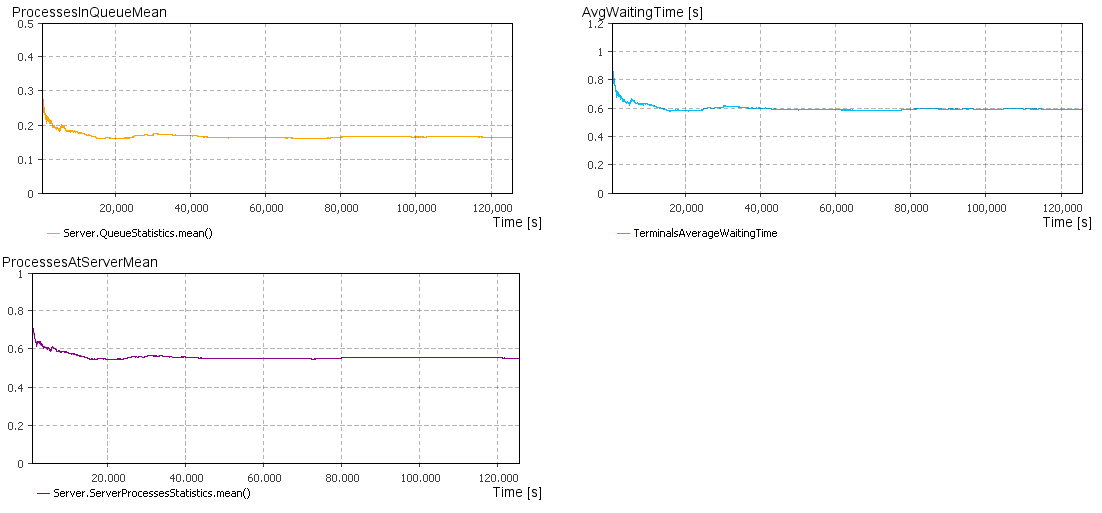
\includegraphics[width=0.9\textwidth]{./images/Simulation_SteadyState}
  \caption{Simulation des CPU Models, mit Steady State}
  \label{fig:SimulationA}
\end{figure}

\begin{figure}[h]
  \centering
  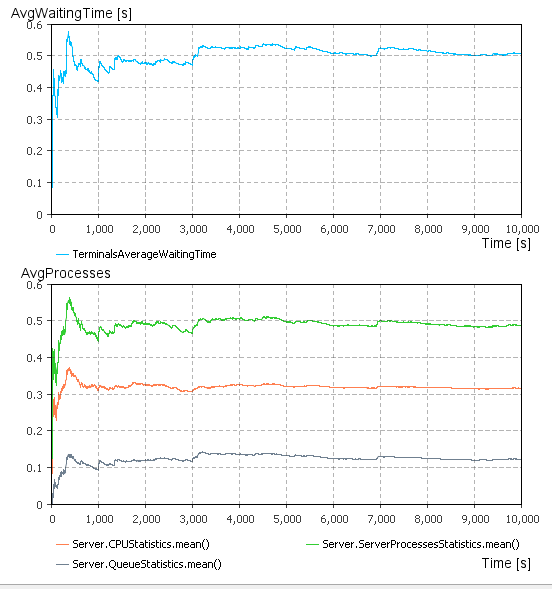
\includegraphics[width=0.9\textwidth]{./images/Simulation_t10000}
  \caption{Simulation des CPU Models, Einschwingvorgang bis $t=10000$}
  \label{fig:Simulation_t10000}
\end{figure}

\begin{figure}[h]
  \centering
  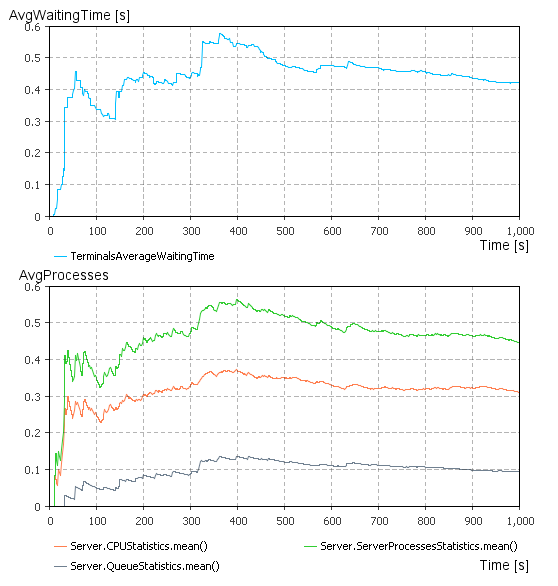
\includegraphics[width=0.9\textwidth]{./images/Simulation_t1000}
  \caption{Simulation des CPU Models, Einschwingvorgang bis $t=1000$}
  \label{fig:Simulation_t1000}
\end{figure}

\begin{figure}[h]
  \centering
  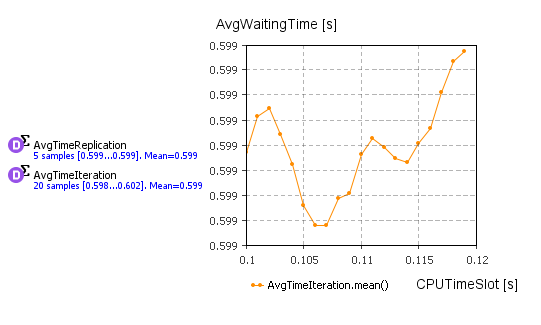
\includegraphics[width=1\textwidth]{./images/ParameterVariationCPUTimeSlot}
  \caption{Parametervariation der Zeitscheibendauer}
  \label{fig:ParametervariationB}
\end{figure}

\begin{figure}[h]
  \centering
  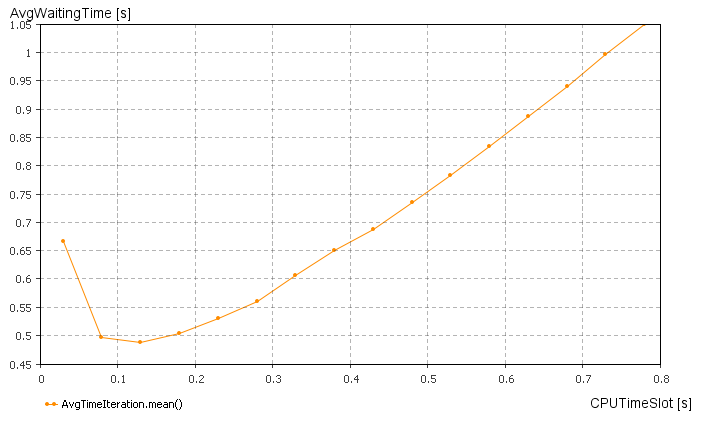
\includegraphics[width=1\textwidth]{./images/ParameterVariationCPUTimeSlot_1}
  \caption{Parametervariation der Zeitscheibendauer}
  \label{fig:ParametervariationB-02}
\end{figure}

\begin{figure}[h]
  \centering
  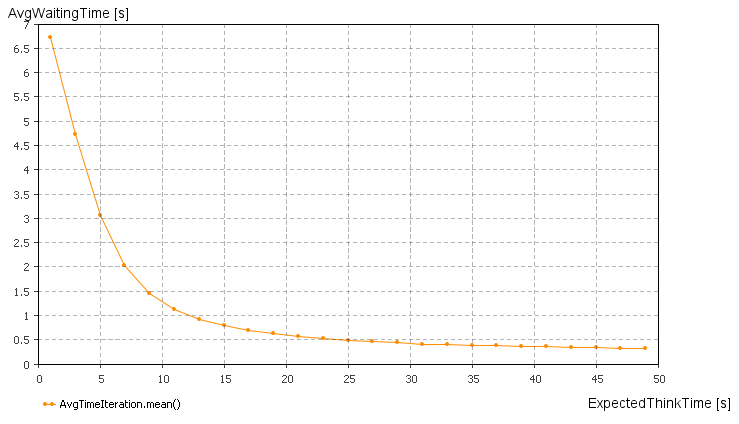
\includegraphics[width=1\textwidth]{./images/ParameterVariationExpectedThinkTime}
  \caption{Parametervariation Erwartete Denkzeit}
  \label{fig:ThinkTime}
\end{figure}

\begin{figure}[h]
  \centering
  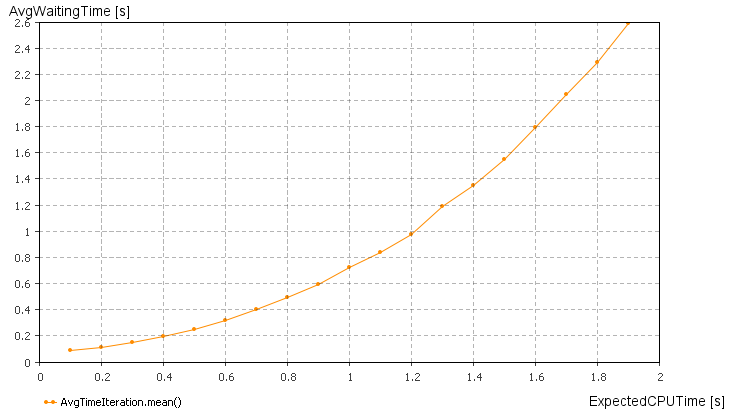
\includegraphics[width=1\textwidth]{./images/ParameterVariationExpectedCPUTime}
  \caption{Parametervariation Erwartete CPU - Zeit}
  \label{fig:CPUTime}
\end{figure}

\begin{figure}[h]
  \centering
  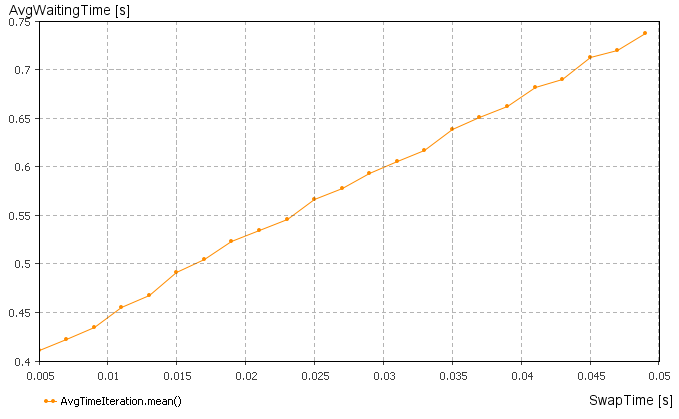
\includegraphics[width=1\textwidth]{./images/ParameterVariationSwapTime}
  \caption{Parametervariation Austausch - Zeit}
  \label{fig:SwapTime}
\end{figure}

\begin{figure}[h]
  \centering
  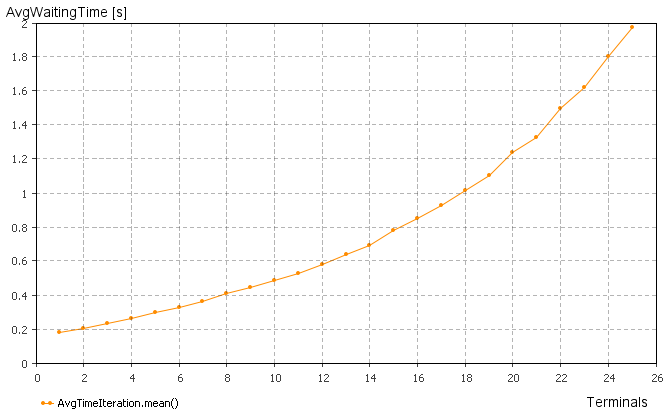
\includegraphics[width=1\textwidth]{./images/ParameterVariationTerminals}
  \caption{Parametervariation Anzahl Terminals}
  \label{fig:TerminalCount}
\end{figure}

\begin{figure}[h]
  \centering
  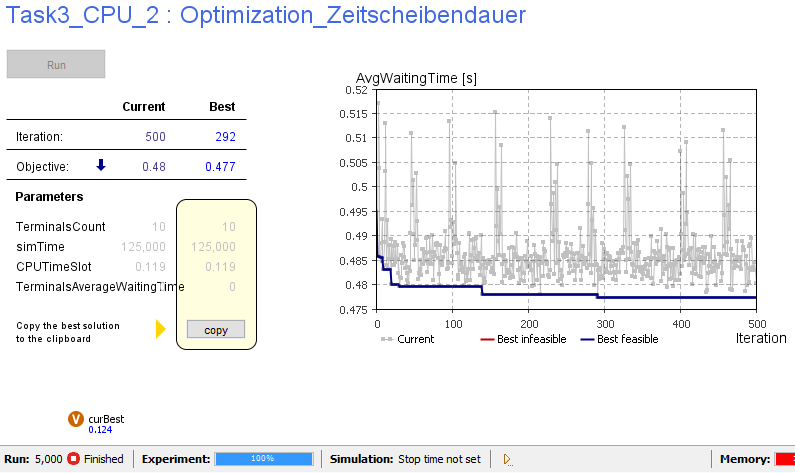
\includegraphics[width=1\textwidth]{./images/Optimization}
  \caption{Optimierung der Zeitscheibendauer}
  \label{fig:OptimizationC}
\end{figure}

\appendix  
\bibliographystyle{plain}
\bibliography{projekt.bib}

\end{document}